%% (Master) Thesis template
% Template version used: v1.4
%
% Largely adapted from Adrian Nievergelt's template for the ADPS
% (lecture notes) project.


%% We use the memoir class because it offers a many easy to use features.
\documentclass[11pt,a4paper,titlepage]{memoir}

%% Packages
%% ========

%% LaTeX Font encoding -- DO NOT CHANGE
\usepackage[OT1]{fontenc}

%% Babel provides support for languages.  'english' uses British
%% English hyphenation and text snippets like "Figure" and
%% "Theorem". Use the option 'ngerman' if your document is in German.
%% Use 'american' for American English.  Note that if you change this,
%% the next LaTeX run may show spurious errors.  Simply run it again.
%% If they persist, remove the .aux file and try again.
\usepackage[english]{babel}

%% Input encoding 'utf8'. In some cases you might need 'utf8x' for
%% extra symbols. Not all editors, especially on Windows, are UTF-8
%% capable, so you may want to use 'latin1' instead.
\usepackage[utf8]{inputenc}

%% This changes default fonts for both text and math mode to use Herman Zapfs
%% excellent Palatino font.  Do not change this.
\usepackage[sc]{mathpazo}

%% The AMS-LaTeX extensions for mathematical typesetting.  Do not
%% remove.
\usepackage{amsmath,amssymb,amsfonts,mathrsfs}

%% NTheorem is a reimplementation of the AMS Theorem package. This
%% will allow us to typeset theorems like examples, proofs and
%% similar.  Do not remove.
%% NOTE: Must be loaded AFTER amsmath, or the \qed placement will
%% break
\usepackage[amsmath,thmmarks]{ntheorem}

%% LaTeX' own graphics handling
\usepackage{graphicx}

%% We unfortunately need this for the Rules chapter.  Remove it
%% afterwards; or at least NEVER use its underlining features.
\usepackage{soul}

%% This allows you to add .pdf files. It is used to add the
%% declaration of originality.
\usepackage{pdfpages}

%% Some more packages that you may want to use.  Have a look at the
%% file, and consult the package docs for each.
%% See the TeXed file for more explanations

%% [OPT] Multi-rowed cells in tabulars
%\usepackage{multirow}

%% [REC] Intelligent cross reference package. This allows for nice
%% combined references that include the reference and a hint to where
%% to look for it.
\usepackage{varioref}

%% [OPT] Easily changeable quotes with \enquote{Text}
%\usepackage[german=swiss]{csquotes}

%% [REC] Format dates and time depending on locale
\usepackage{datetime}

%% [OPT] Provides a \cancel{} command to stroke through mathematics.
%\usepackage{cancel}

%% [NEED] This allows for additional typesetting tools in mathmode.
%% See its excellent documentation.
\usepackage{mathtools}

%% [ADV] Conditional commands
%\usepackage{ifthen}

%% [OPT] Manual large braces or other delimiters.
%\usepackage{bigdelim, bigstrut}

%% [REC] Alternate vector arrows. Use the command \vv{} to get scaled
%% vector arrows.
\usepackage[h]{esvect}

%% [NEED] Some extensions to tabulars and array environments.
\usepackage{array}

%% [OPT] Postscript support via pstricks graphics package. Very
%% diverse applications.
%\usepackage{pstricks,pst-all}

%% [?] This seems to allow us to define some additional counters.
%\usepackage{etex}

%% [ADV] XY-Pic to typeset some matrix-style graphics
%\usepackage[all]{xy}

%% [OPT] This is needed to generate an index at the end of the
%% document.
%\usepackage{makeidx}

%% [OPT] Fancy package for source code listings.  The template text
%% needs it for some LaTeX snippets; remove/adapt the \lstset when you
%% remove the template content.
\usepackage{listings}
\lstset{language=TeX,basicstyle={\normalfont\ttfamily}}

%% [REC] Fancy character protrusion.  Must be loaded after all fonts.
\usepackage{microtype}

%% [REC] Nicer tables.  Read the excellent documentation.
\usepackage{booktabs}


%% Our layout configuration.  DO NOT CHANGE.
%% Memoir layout setup

%% NOTE: You are strongly advised not to change any of them unless you
%% know what you are doing.  These settings strongly interact in the
%% final look of the document.

% Dependencies
\usepackage{ETHlogo}

% Turn extra space before chapter headings off.
\setlength{\beforechapskip}{0pt}

\nonzeroparskip
\parindent=0pt
\defaultlists

% Chapter style redefinition
\makeatletter

\if@twoside
  \pagestyle{Ruled}
  \copypagestyle{chapter}{Ruled}
\else
  \pagestyle{ruled}
  \copypagestyle{chapter}{ruled}
\fi
\makeoddhead{chapter}{}{}{}
\makeevenhead{chapter}{}{}{}
\makeheadrule{chapter}{\textwidth}{0pt}
\copypagestyle{abstract}{empty}

\makechapterstyle{bianchimod}{%
  \chapterstyle{default}
  \renewcommand*{\chapnamefont}{\normalfont\Large\sffamily}
  \renewcommand*{\chapnumfont}{\normalfont\Large\sffamily}
  \renewcommand*{\printchaptername}{%
    \chapnamefont\centering\@chapapp}
  \renewcommand*{\printchapternum}{\chapnumfont {\thechapter}}
  \renewcommand*{\chaptitlefont}{\normalfont\huge\sffamily}
  \renewcommand*{\printchaptertitle}[1]{%
    \hrule\vskip\onelineskip \centering \chaptitlefont\textbf{\vphantom{gyM}##1}\par}
  \renewcommand*{\afterchaptertitle}{\vskip\onelineskip \hrule\vskip
    \afterchapskip}
  \renewcommand*{\printchapternonum}{%
    \vphantom{\chapnumfont {9}}\afterchapternum}}

% Use the newly defined style
\chapterstyle{bianchimod}

\setsecheadstyle{\Large\bfseries\sffamily}
\setsubsecheadstyle{\large\bfseries\sffamily}
\setsubsubsecheadstyle{\bfseries\sffamily}
\setparaheadstyle{\normalsize\bfseries\sffamily}
\setsubparaheadstyle{\normalsize\itshape\sffamily}
\setsubparaindent{0pt}

% Set captions to a more separated style for clearness
\captionnamefont{\sffamily\bfseries\footnotesize}
\captiontitlefont{\sffamily\footnotesize}
\setlength{\intextsep}{16pt}
\setlength{\belowcaptionskip}{1pt}

% Set section and TOC numbering depth to subsection
\setsecnumdepth{subsection}
\settocdepth{subsection}

%% Titlepage adjustments
\pretitle{\vspace{0pt plus 0.7fill}\begin{center}\HUGE\sffamily\bfseries}
\posttitle{\end{center}\par}
\preauthor{\par\begin{center}\let\and\\\Large\sffamily}
\postauthor{\end{center}}
\predate{\par\begin{center}\Large\sffamily}
\postdate{\end{center}}

\def\@advisors{}
\newcommand{\advisors}[1]{\def\@advisors{#1}}
\def\@department{}
\newcommand{\department}[1]{\def\@department{#1}}
\def\@thesistype{}
\newcommand{\thesistype}[1]{\def\@thesistype{#1}}

\renewcommand{\maketitlehooka}{\noindent\ETHlogo[2in]}

\renewcommand{\maketitlehookb}{\vspace{1in}%
  \par\begin{center}\Large\sffamily\@thesistype\end{center}}

\renewcommand{\maketitlehookd}{%
  \vfill\par
  \begin{flushright}
    \sffamily
    \@advisors\par
    \@department, ETH Z\"urich
  \end{flushright}
}

\checkandfixthelayout

\setlength{\droptitle}{-48pt}

\makeatother

% This defines how theorems should look. Best leave as is.
\theoremstyle{plain}
\setlength\theorempostskipamount{0pt}

%%% Local Variables:
%%% mode: latex
%%% TeX-master: "thesis"
%%% End:


%% Theorem environments.  You will have to adapt this for a German
%% thesis.
%% Theorem-like environments

%% This can be changed according to language. You can comment out the ones you
%% don't need.

\numberwithin{equation}{chapter}

%% German theorems
%\newtheorem{satz}{Satz}[chapter]
%\newtheorem{beispiel}[satz]{Beispiel}
%\newtheorem{bemerkung}[satz]{Bemerkung}
%\newtheorem{korrolar}[satz]{Korrolar}
%\newtheorem{definition}[satz]{Definition}
%\newtheorem{lemma}[satz]{Lemma}
%\newtheorem{proposition}[satz]{Proposition}

%% English variants
\newtheorem{theorem}{Theorem}[chapter]
\newtheorem{example}[theorem]{Example}
\newtheorem{remark}[theorem]{Remark}
\newtheorem{corollary}[theorem]{Corollary}
\newtheorem{definition}[theorem]{Definition}
\newtheorem{lemma}[theorem]{Lemma}
\newtheorem{proposition}[theorem]{Proposition}

%% Proof environment with a small square as a "qed" symbol
\theoremstyle{nonumberplain}
\theorembodyfont{\normalfont}
\theoremsymbol{\ensuremath{\square}}
\newtheorem{proof}{Proof}
%\newtheorem{beweis}{Beweis}


%% Helpful macros.
%% Custom commands
%% ===============

%% Special characters for number sets, e.g. real or complex numbers.
\newcommand{\C}{\mathbb{C}}
\newcommand{\K}{\mathbb{K}}
\newcommand{\N}{\mathbb{N}}
\newcommand{\Q}{\mathbb{Q}}
\newcommand{\R}{\mathbb{R}}
\newcommand{\Z}{\mathbb{Z}}
\newcommand{\X}{\mathbb{X}}

%% Fixed/scaling delimiter examples (see mathtools documentation)
\DeclarePairedDelimiter\abs{\lvert}{\rvert}
\DeclarePairedDelimiter\norm{\lVert}{\rVert}

%% Use the alternative epsilon per default and define the old one as \oldepsilon
\let\oldepsilon\epsilon
\renewcommand{\epsilon}{\ensuremath\varepsilon}

%% Also set the alternate phi as default.
\let\oldphi\phi
\renewcommand{\phi}{\ensuremath{\varphi}}


%% Make document internal hyperlinks wherever possible. (TOC, references)
%% This MUST be loaded after varioref, which is loaded in 'extrapackages'
%% above.  We just load it last to be safe.
\usepackage[linkcolor=black,colorlinks=true,citecolor=black,filecolor=black]{hyperref}


%% Document information
%% ====================

\title{Title of Thesis}
\author{S. Tudent}
\thesistype{Master Thesis}
\advisors{Advisors: Prof.\ Dr.\ A. D. Visor, Dr.\ P. Ostdoc}
\department{Department of Computer Science}
\date{January 19, 2038}

\begin{document}

\frontmatter

%% Title page is autogenerated from document information above.  DO
%% NOT CHANGE.
\begin{titlingpage}
  \calccentering{\unitlength}
  \begin{adjustwidth*}{\unitlength-24pt}{-\unitlength-24pt}
    \maketitle
  \end{adjustwidth*}
\end{titlingpage}

%% The abstract of your thesis.  Edit the file as needed.
\begin{abstract}
 Our implementation of a verified instruction selection pipeline from a subset of LLVM IR, produced by the Lean compiler, to ARM machine code is a first step toward strengthening trust in Lean’s translation process and proof by reflection, with the long-term goal of a fully verified Lean theorem proving infrastructure. The Lean interactive theorem prover plays a crucial role in formal verification. While its kernel has been verified, its compiler remains largely unverified. This is concerning for proof by reflection, where computations act as certificates for proofs, making compiler correctness essential for trustworthiness. We counteract this gap by implementing and verifying an instruction selection pass that translates LLVM IR to ARM assembly in Lean4 while preserving program semantics. We target a subset of LLVM IR commonly produced by the Lean compiler—load/store operations and integer arithmetic— and translate it to an ISA exhibiting formal correctness guarantees. Our implementation leverages formal models of LLVM and ARM and incorporates peephole optimization patterns for improved instruction selection. By utilizing bv\_ decide, a tactic within Lean allowing for automated bit vector reasoning, we gain significantly more proof automation compared to other projects like CompCert. The primary results of this work establish that any translation from LLVM IR to ARM machine code using our pipeline provides formal correctness guarantees proven in Lean.   
 
\end{abstract}


%% TOC with the proper setup, do not change.
\cleartorecto
\tableofcontents
\mainmatter

%% Your real content!
% Some commands used in this file
\newcommand{\package}{\emph}

\chapter{Introduction}
Lean [1,2] is a proof assistant and purely functional programming language, providing users with a tool for interactive theorem proving and software development. Lean itself offers a compiler that produces fast native code, which is written by translating Lean source code into Lean's core language, which will then be subsequently lowered to LLVM IR and then via the LLVM backend compiled into machine code specific for the target architecture [3]. As this compilation path leverages the optimizations and backend provided by LLVM to produce fast code, it heavily relies on the LLVM compiler toolchain. 

The Lean compiler is used not only to produce executables from Lean source code but is also crucial in a style of proof called 'proof by reflection' where a computation is executed, and the output of the computation is used as a certificate for a proof. This use of the compiler for proving makes verifying the Lean compiler an important research target, since the trustworthiness of fast proof by reflection in Lean hinges on the trustworthiness of its compiler toolchain. However, LLVM's large codebase with numerous optimization passes makes such a verification complex [4]. Full verification of Lean's compilation process is unlikely as it requires a fully verified LLVM compiler, while verification efforts for LLVM currently only cover its higher-level stacks around LLVM-IR (e.g., Vellvm [5]) and also only exist in ROCQ [6]. As a first step towards a verified Lean backend, with an eye towards providing trustworthy proof by reflection for Lean, this work proposes to develop a verified instruction selection pipeline that translates LLVM IR into an ISA, here choosen to be RISC-V, to produce fast machine-specific code. This verified instruction selection pipeline aims to provide formal guarantees that the RISC-V assembly code generated from Lean source programs stays semantically equivalent to the LLVM IR representation of the program in Lean’s core language. While the actual connection to Lean’s core language is a non-goal, we will focus in this project on the subset of LLVM-IR that would typically be generated by Lean, e.g., LLVM-IR consisting of load/store operations plus integer arithmetic.

To implement such a formally verified instruction selection pass, we leverage and build upon existing RISC-V and LLVM specifications and publically available datasets of peephole optimizations (e.g., from the GCC compiler backend). The Lean-MLIR project [7] already provides a semantic model of the arithmetic fragment of LLVM, which can be used as a starting point for the needed LLVM semantics. RISC-V semantics are also well-defined and given in a formal specification by the SAIL project1 [8]. Additionally, compiler backends like in GCC or LLVM provide a repository with an extensive collection of peephole optimization patterns, which we could adapt to an LLVM-like abstract ISA and leverage to write our verified instruction selection pipeline to generate optimized machine code.

We shall use the insights from projects like Peek [9], which implements a peephole optimization pass for x86 in CompCERT [10]. In this work, we will integrate the use of verification tools to formally show the semantic equivalence of the LLVM IR instructions to be lowered and our generated RISC-V lowering. Leveraging bv\underline decide [7], the first fully verified SMT solver natively integrated into an interactive theorem prover, we gain significantly more proof automation compared to other projects like CompCert. Therefore, we shall attempt to automate many of these proofs using SMT-LIB compatible proof automation ( bv \underline decide) and Lean’s extensive bit vector library.


\chapter{Background}
In the following section we will introduce the topics relevant to understand the work of this thesis. We will first
focus on the LLVM project and on the design of compilers. Then we will focus on theorem proving in Lean and the formalization of language semantics for LLVM IR and the RISC-V ISA.

\section {The LLVM Ecosystem}
%sources [1] 2022_Yilin paper 
% [2] Peter Müller talk 
%in general and then LLVM IR and then MLIR especially 
\subsection{ LLVM }
The LLVM (Low-Level Virtual Machine) project is an open-source compiler infrastructure maintained by a large, active developer community. It provides a collection of reusable and modular compiler and toolchain technologies[1].  As of today, LLVM is foundational to the compilation of many modern programming languages, including C, Rust, and Haskell.

At the core of the LLVM project is its compiler intermediate representation, LLVM IR. LLVM IR is a target-independent, low-level language that acts as an intermediate abstraction layer between the source language and machine-specific assembly code. A compiler IR is characterized by being more abstract than machine code, making it easier to optimize since more of the program's structure is preserved. At the same time, it is less abstract than high-level source languages, which contain language-specific constructs.
This balance makes IRs ideal for implementing language-agnostic optimizations that can be reused across multiple source and target languages. The concept of IRs as an abstraction layer for expressing shared properties has gained attention not only in compiler design but has also been adopted in projects aimed at building reusable tools e.g. verification frameworks.[2]

In LLVM-based compilers, LLVM IR serves as the primary  representation of programs throughout the compilation chain. A compilation path leveraging LLVM can be decoupled into three phases:
- Frontend: It translates source code into LLVM IR and must be provided by the compiler engineer of the source language.

- Optimization: A series of transformation and analysis passes is performed on LLVM IR and is provided by LLVM toolchain. Currently XY are supported in LLVM.

- Code generation: After language-agnostic optimization on LLVM IR, the program is lowered via an LLVM backend to machine code.

The architectural separation between language-specific frontends and language-independent optimization and code generation in LLVM enables the reuse of its middle-end and backend components across a wide range of programming languages. 

An important feature of LLVM IR that makes it a suitable foundation for analysis and optimization passes is its use of Single Static Assignment (SSA) form. In SSA, each variable is assigned exactly once, resulting in a unique definition point for every variable. This property simplifies data flow analysis and, consequently, enables more effective compiler optimizations.

Optimization within the LLVM is performed using a modular approach, where code optimizations are structured in passes.
 XY (TO DO) percentage of these optimization passes operate directly on LLVM IR. For example, InstCombine is a transformation pass that rewrites sequences of IR instructions into optimized, more efficient equivalents, which is known as performing peephole optimizations (see chaptre xy).

 [to do: list of relevant passes to this thesis:
  DCE, CSE and InstCombine, DAGCombine]

To apply the passes LLVM offers its users a set of built-in optimization levels corresponding to a set of optimization passes ( -O1 through -O3 ). Additionally, LLVM provides users with the ability to write custom passes or apply a tailored sequence of existing passes. Using LLVM’s optimizer tool, opt, users can execute a customized pass pipeline as follows:

[opt -pass1 -pass2 ... [input file] -o [output file]]

The opt tool can print the optimized output to the command line, allowing users to inspect and visualize the effects of applied optimizations. This functionality offers an interactive way to experiment with LLVM’s optimization infrastructure and serves as inspiration for designs in which verified passes could be selectively applied and observed.

\subsection{MLIR}
%[sources: https://lup.lub.lu.se/luur/download?func=downloadFile&recordOId=9146373&fileOId=9146374, MLIR.llvm.org 
%]
The strength of LLVM lies in its modular and reusable design, which is tightly coupled to its intermediate representation. The design using an IR enables the reuse of optimization passes and backend components across the compilation of a diverse range of programming languages. MLIR (Multi-Level Intermediate Representation), a subproject within the LLVM ecosystem, extends these principles to support domain-specific compilation.
For this purpose, unlike LLVM IR, which offers a single IR, MLIR provides an infrastructure that supports multiple IRs, referred to as dialects. These dialects are logically separated namespaces that support operations, types, and attributes relevant to a specific domain or abstraction level but overall are all unified within single hybrid IR. As the name suggests, MLIR is designed to support a multi-level IR, where various levels of abstraction are represented by these dialects tailored to a specific purpose. High-level dialects typically represent constructs from source languages or high level domain- specfic operations e.g. accelarator specfic high-level operations, while low-level dialects are designed to model operations close to target-dependent machine instructions e.g register architectures or explicit DMA insertions. A program in MLIR can use different dialects, allowing different parts of the program to be represented in a way suited to their respective abstraction levels. Each dialect in MLIR follows a consistent syntax that makes the , where operations are prefixed with a dotted prefix  that reflects the dialect namespace.
The following is a multiplication function in MLIR using the func and arith dialects, which represent functions and arithmetic instructions.
\begin{figure}[ht]
\centering
\begin{lstlisting}[language=mlir, basicstyle=\ttfamily\small]
module {
  func.func @mul() -> i32 {
    %a = arith.constant 19 : i32 
    %b = arith.constant 10 : i32 
    %c = arith.muli %a, %b : i32 
    return %c : i32
  }
}
\end{lstlisting}
\caption{ MLIR function that performs a multiply. Functions are represented as operations in the func dialect, arithmetic operations using the arith dialect.}
\label{fig:mlir-addition}
\end{figure}

A core technique in MLIR is the concept of performing progressive lowerings. In this process, a source program is incrementally transformed through a series of dialects. This transformation continues until the program reaches a low-level form that is suitable for final code generation. 

During this progressive lowering, optimizations can be applied. MLIR adopts LLVM’s pass-based optimization model. Optimization and analysis passes in MLIR are dialect-aware, meaning they operate specifically on the operations and types defined within each dialect and therefore perform optimizations tuned for that specific abstraction level.
LLVM IR itself is included as a dialect within MLIR, which allows programs represented in MLIR to be lowered to LLVM IR and vice versa.
LLVM IR can be lowered to its MLIR dialect representation by applying a compiler pass represented by --transform-llvmir. Conversely, any MLIR program can be exported to LLVM IR using the  -convert-to-dialect-tollvm pass provided by the MLIR toolchain.

An example of progressivly lowering the multiplication function in listing, by applying --convert-arith-to-llvm pass is shown below. The operations in the arith dialect are lowered to the llvm ir dialect while func operations remain untransformed. 
\begin{figure}[ht]
\centering
\begin{lstlisting}[language=mlir, basicstyle=\ttfamily\small]
module {
  func.func @mul() -> i32 {
    %0 = llvm.mlir.constant(19 : i32) : i32
    %1 = llvm.mlir.constant(10 : i32) : i32 
    %2 = llvm.mlir.constant(40 : i32) : i32
    return %2 : i32
  }
}
\end{lstlisting}
\caption{ Progressive lowering: Converting arith operations to LLVM operations while Func operations are not lowered in this phase. }
\label{fig:mlir-addition}
\end{figure}
By applying an additional -convert-func-to-llvm and -canonicalize pass, the resulting mlir code is listed in XY. 
\begin{figure}[ht]
\centering
\begin{lstlisting}[language=mlir, basicstyle=\ttfamily\small]
module attributes {llvm.data_layout = ""} { 
 llvm.func @main() -> i32 {
    %0 = llvm.mlir.constant(190 : i32) : i32 
    llvm.return %0 : i32
    } 
}
\end{lstlisting}
\caption{ Progressive lowering: Converting func operations to LLVM operations and canocnliaze. }
\label{fig:mlir-addition}
\end{figure}
These lowering phases illustrate the use of MLIR as a multi-level IR, where a program is progressively lowered through a sequence of passes applied to a hybrid IR composed of multiple dialects.

The conversions between MLIR IRs and LLVM IR enable LLVM IR to be ported into the MLIR LLVM dialect and conversely, allow the LLVM backend to generate machine code from MLIR by converting it to LLVM IR.

LLVM and with it MLIR are compiler frameworks that leverage the use of intermediate representations and targeted optimizations that exhibit returns across many targets.  A compiler stack is commonly composed of a series of lowerings and transformations that translate a source program into machine-specific assembly code. A key stage in this process is instruction selection, which is preceded by IR optimizing passes and followed by target-specific optimizations. 

\section{Instruction Selection \& Optimization}
\subsection {Instruction Selection}
During the compilation process, a source program passes through multiple transformation stages before it is converted into an executable. Code generation is a key phase in compiler backends where machine code is produced from the intermediate representation (IR) of the program. Instruction selection is usually located within the code generator and is performed before instruction scheduling and register allocation. During Instruction selection high-level IR operations are converted into concrete instructions defined by the target architecture’s Instruction Set Architecture (ISA), or into a lower-level IR depending on the compiler's design.
 This translation is non-trivial, as a single IR instruction may correspond to multiple possible sequences of machine instructions each offering different trade-offs in terms
of performance, code size, or resource usage. 

The IR often includes abstract operations that do not map one-to-one to the instructions available in the ISA. In many cases, the ISA supports a narrower set of operations compared to those represented in the IR e.g RISC-V does not supported a neg instruction while LLVM IR does. Therefore, instruction selection must decompose complex IR operations into semantically equivalent sequences of machine instructions while preserving the original program behavior.

[TO DO : give an example lowering if icmp ]

Instruction selection is critical,as it contributes to how the high-level program semantics are preserved in the final executable. If the mapping from IR instruction to machine code instruction is semantically incorrect, the resulting executable will fail to correctly implement the source program.

[to do: write baout instruction selection and tabel gen files etc how they are matched ]
In modern compiler frameworks such as LLVM, instruction selectors are typically implemented using pattern matching mechanisms. Instruction selectors rely on a set of predefined rules that match specific IR instruction patterns and replace them with the corresponding target machine instructions, when that pattern is found in the program. The instruction selection process can also be formulated as a graph covering problem. In the graph-based approach, the IR is transformed into a graph representation, where instruction selection involves covering this graph with tiles that represent machine instructions. The goal is to find a covering that minimizes a defined cost metric e.g such as execution time or instruction count. Depending on the complexity of instruction selection, the compiler may produce suboptimal code. Due to the lowering process from one language to another inefficiencies can be introduced or new optimization opportunities arise due to the structure of the target-specific machine code. 
[TO DO : ACTUALLY DOUBLE CHECK THIS ]
As a result, compilers often include peephole optimization passes after instruction selection. Peephole optimizations are introduced in detail in the next subsection after introdcuing Risc-V, the target architecture ISA ued in our instruction selection.

\subsection{Peephole Optimizations}
Peephole optimization is a fundamental technique in a compilers optimization toolkit [3 peek]e.g employed in production compilers like GCC (a C compiler) and LLVM. Peephole optimizations involves analyzing short sequences of instructions and transforming them into semantically equivalent but more efficient sequences.  Peephole rewrites focus on a small, localized section of the code ("a peephole")  and transform few instructions into semanitcally equivalent but optimized instruction sequences. Common types of peephole optimization include constant folding (replacing calculations on constants with their result) and strength reduction (replacing expensive operations with cheaper ones). When perforemd on machine cde level they contain architecutre specific optimzations e.g. choosing diffrent instructions to maximize the use of the avaiable functional units. Peephole optimizations individually focus on a small scope, but  applied throughout a program significantly improve performance and reduce code size. Additionally peephole optimizations are emplyoed in canonciluzation passes (see listing of mlir above), to rewrite code into a standard or simplified form. The LLVM InstCombine pass is peephole optimization pass that performs IR-to-IR rewrites and  [TO DO MORE facts about InstCombine ]
 \begin{lstlisting}[language=Python, caption=unoptimized IR instruction sequence]
    %v1 = llvm.and %X, %Y
    %v2 = llvm.or %X, %Y
    %v3 = llvm.add %v1, %v2
\end{lstlisting}
 \begin{lstlisting}[language=Python, caption= peephole optimized IR instruction sequence ]
 %v3 = llvm.add %X, %Y
\end{lstlisting}
 [TO DO INASERT GRAPHIC OF PEEPHOLE OPTIMIZATION PASS ]
 Traditionally, peephole optimization is implemented using pattern-based rewriting. The compiler matches a predefined find pattern — which specifies a particular instruction sequence — and replaces it with a corresponding replace - pattern that yields semantically equivalent but performance optimized sequence. Peephole optimization is performed at various stages of the compilation pipeline, such as on the intermediate representation level to improve the IR after high-level transformations or at the assembly level to refine the final machine code.
\section {RISC-V 64}
\subsection{ ISA}
The target language of our instruction selection will be lowered  is RISC-V, an open instruction set architecture developed at the University of Berkley. As the name suggests RISC-V is based on the reduced instruction set computer principle (RISC), where the ISA exhibits potentially many but simple instructions in comparison to CISC architectures.  RISC-V compromises an integer base ISA that comes with various added extensions allowing for a modular and domain-specific design of the ISA. RISC-V is available as a 32-bit (RV32) and 64-bit (RV64) architecture version while there are current efforts for  larger address space architectures like  RV128. 

The RISC-V base ISA specifies instructions for logic operations like integer manipulation, address calculation, control flow, and memory allowing for implementation of a simple general-purpose computer. Extensions like the bit manipulation extension (e.g ZBB)  supplement the base ISA and target code size reduction or performance improvement. The ZBB extension is defined for RV32 and RV64 (and follows the convention specified for RV64).
\subsection{ ISA Semantics}
\section {Lean}
\subsection{ Lean 4 }
\subsection{ Proving in Lean }
\subsection{ Bit Vector reasoning in Lean }
\section {Lean-Mlir}
\chapter{Framework Set-Up}
This chapter describes the infrastructure used to model our instruction selection and optimization pass. We begin by modeling RISC-V as dialect within the Lean-MLIR project and leveraging the existing LLVM IR dialect. Next, we present the hybrid RISC-V and LLVM IR dialect and explain its relevance to our instruction selection approach. We then introduce the verified tools that allow us to apply formally verified transformations to LLVM IR programs. Finally, we state our overall correctness theorem.

\section{RISC-V dialect\& semantics}
\subsection{ RISC-V semantics from Sail}

\section{LLVM IR dialect\& semantics}

Lean-MLIR provides an LLVM IR dialect model in Lean that mirrors the arithmetic fragment of LLVM IR. The instructions are encoded as operations within the LLVM IR dialect, which mirrors the MLIR LLVM IR dialect and can be instantiated with any bit vector width allowed by the LLVM language reference. Additionally, Lean-MLIR provides the framework to assign a semantic denotation to each operation, thereby modeling the semantics of the LLVM IR dialect. The LLVM IR dialect model in Lean, which we leverage, supports the following LLVM IR in figure XY, including the overflow flags nsw, nuw, and the exact flag. 

When the nsw (no signed wrap) and nuw (no unsigned wrap) flags are set, signed and unsigned overflows are considered poison. The exact flag, which is supported for certain operations in LLVM, indicates whether rounding or shifting behavior should be treated as a special value, called \textit{poison} (see chaptre bellow), if the computation is not exact, meaning a non-zero rounding or e.g. a reminder for division is present.
$[TO DO: figure of LLVM IR instructions in Lean-MLIR]$

The Lean-MLIR framework provides a parser in Lean which allows users to provide a LLVM IR program written in a MLLIR-generic syntax (see figure XY), which then parsers it into the Lean internal representation, where each program is defined as a sequences of well-typed computations and expression. An LLVM IR dialect program can be modelled as shown in figure XY. This enables users to write LLVM IR dialect seuqences in the Lean using syntax that they are familiar with from MLIR compiler developement. 

\begin{figure}
\begin{minipage}{1\textwidth}
\begin{lstlisting}
def example_llvm_function := [llvm|
{
^0(%arg317 : i32):
  %0 = llvm.mlir.constant(1 : i32) : i32
  %1 = llvm.shl %0, %arg317 : i32
  %2 = llvm.and %1, %0 : i32
  "llvm.return"(%2) : (i32) -> ()
}
   
\end{lstlisting}
\end{minipage}
\caption{semantics of LLVM IR shl instruction defined by Lean-MLIR}
\label{fig:LLVMIR-SEMANTICS-SHL}
\end{figure}
\subsection{LLVM IR semantics}
The LLVM IR dialect in Lean-MLIR models the LLVM IR semantics using the bit vector domain in Lean. To faithfully represent the language constructs supported in LLVM IR, the semantics use a dedicated \textit{PoisonOr} structure that is either a bit-vector value or a poison value, which underlying is modeled as a monadic \textit{none}. This distinction is crucial, as the LLVM semantics exhibit undefined behavior that must be taken into account during the lowering of a program and require careful reasoning when defining correctness of a lowering from LLVM IR. (more on this in a chapter XY). 
Below are examples on how the semantics for an LLVM IR instruction is defined within Lean-MLIR. Each instruction is modeled as an operation on a dependently typed bit vector \textit{IntW w}, which describes a bit vector of width \textit{w}.

%def lshr {w : Nat} (x y : IntW w) (flag : ExactFlag := {exact := %false}) : IntW w := do
  %let x' ← x
  %let y' ← y
  %if flag.exact ∧(x' >>> y') <<< y' ≠ x' then
    %.poison
  %else
    %lshr? x' y'
   
\begin{figure}
\begin{minipage}{0.45\textwidth}
\begin{lstlisting}
def lshr? {n} (op1 : BitVec n) (op2 : BitVec n) : IntW n :=
  if op2 >= n
  then .poison
  else .value (op1 >>> op2)
\end{lstlisting}
\end{minipage}
\caption{semantics of LLVM IR shl instruction defined by Lean-MLIR}
\label{fig:LLVMIR-SEMANTICS-SHL}
\end{figure}

\textbf{Undefined Behaviour in LLVM IR and its Lean-MLIR model }[TO DO: still have not understood everything]

LLVM IR defines two forms of undefined behavior (UB), which are distinguished by their origin and how they are treated by the compiler. Immediate undefined behavior is the strictest form and represents operations that typically result in a trap at runtime on most processors supported by LLVM, e.g., division by zero. When immediate UB occurs in an LLVM IR program the compiler is not required to preserve any of its observable behavior and in many cases it can lead to the program crashing or throwing an exception [llvm language reference]. Conceptually it allows for very aggressive optimizations where the semantics of the program don't need to be preserved because of UB.

In contrast, LLVM IR also defines a model known as deferred UB, which contains \textit{undef} values and \textit{poison} values. Deferred UB involves operations where the result is not well-defined by the language, but executing the operation itself might not immediately crash the program. Deferred UB differs from immediate UB in that the compiler is permitted to speculate about their semantics and continue execution and optimization. According to the LLVM language reference deferred UB should be used for operations where the semantics across processors differ but do not cause a CPU trap. Therefore, a \textit{ undef} or \textit{poison} value indicates that LLVM does not assign precise semantics to the corresponding operation. This design choice gives the compiler a way to indicate that an operations is mathematically not well-defined but has an implementation on machine architectures e.g  shifting by a value greater than the bit width of the operand. The shift operation in figure XY resolves to a poison value, depending on the processor architecture this then resolves to a concrete value. This means that the compiler can proceed with the code execution speculating about the concrete value.
\begin{figure}
\begin{minipage}{0.45\textwidth}
\begin{lstlisting}
define i32 @poison_shift(i32 %arg) {
  %mask = and i32 %arg, 31
  %shift = shl i32 %arg, %mask
  ret i32 %shift
}
     }
\end{lstlisting}
\end{minipage}
\caption{Shift resulting in a poison value.}
\label{fig:LLVMIR-SEMANTICS-SHL}
\end{figure}

This allows for optimizations like hoisting operations out of loops that would otherwise be impossible due to the potential for undefined behavior at the point where the hoisted operation is executed. LLVM defines certain operations, such as branching or division by zero, where an input with deferred UB is converted into immediate UB for the program. 
Thus, if such an instruction completes successfully, we implicitly know that none of its inputs exhibited UB else immediate UB would have been indicated. In addition to poison values, which propagate through instructions (e.g., an add on a poison value again resolves to poison) there are \textit{undef} values.[john Regehr paper taming ub in llvm ] These can be mentally modeled as reading from uninitialized memory, where each access may yield a different result.
\begin{figure}
\begin{minipage}{0.45\textwidth}
\begin{lstlisting}
define i64 @divzero(i64 %arg) {
    entry:
      %0 = div i64 %arg undef
      ret %0
}
     }
\end{lstlisting}
\end{minipage}
\caption{Deffered UB in div resolves to immediate UB}
\label{fig:LLVMIR-SEMANTICS-SHL}
\end{figure}

\begin{figure}
\begin{minipage}{0.45\textwidth}
\begin{lstlisting}
define i64 @add_eq?_shl(i64 %arg) {
    entry:
      %0 = add i64 %arg %arg
      %1 = shl i64 %arg , 2
      ret icmp eq %0 %1
     }
\end{lstlisting}
\end{minipage}
\caption{LLVM IR function}
\label{fig:LLVMIR-SEMANTICS-SHL}
\end{figure}

To the reader as well as to developers, it might seem obvious that this equality check should evaluate to true. However, this does not hold. If the argument to the function is an undef value, each access might resolve to a different value. Additionally, if the argument is poison, the poison value will taint \textit{\%0} and \textit{\%1}, propagating poison to both.

Overall, LLVM's undefined behavior can be modeled hierarchically, where \textit{undef} represents the weakest form of undefined behavior.

\textit{\textbf{immediate  UB $\vartriangleright$ poison $\vartriangleright $ undef $\vartriangleright$ concrete value.}}

In our work, we leverage the UB model as defined in Lean-MLIR, where no distinction is made between immediate UB and deferred UB; both are modeled using poison values. The instructions within the LLVM IR  fragment modelled in Lean-MLIR and used in this thesis that produce immediate UB are the division and reminder operation. for the LLVM IR optimization pass we therefore manullay check that the rewrite only triggers UB if the original instruction sequences does. For lowering the instructions we follow LLVM's approach as described in Chaptre 5.  Current efforts on Lean-MLIR  work refining the handling of UB. Adapting our current UB model to support more precise UB handling would not pose a significant challenge because, looking at the UB value lattice, an immediate UB can be replaced by a poison value. Especially for code generation, lowering an immediate UB to the same as a poison value is allowed. Besides that, the UB model does not affect the core contributions of this thesis. (see section where define correctness statement).
\section{Hybrid Dialect: LLVM IR and RISC-V}


\section{Verified Peephole Rewriting Infrastrucutre }
Instruction selection and code optimizations are crucial program transformations, and each transformation can conceptually be formalized as a rewrite. Lean-MLIR provides a peephole rewriter that applies a single rewrite rule to sequences of computations and expressions derived from an input LLVM IR program. When the rewriter successfully applies a rewrite, the accompanying correctness proof ensures that the program's semantics are preserved.
Originally, the rewriting infrastructure in Lean-MLIR supported only a single peephole rewrite. We extended this infrastructure to support the application of a sequence of rewrites. The extended rewriter can process a dependently typed list of optimization patterns and iterate over an input program by attempting to apply each rewrite in the list.
The design of the Lean-MLIR rewriter supports pattern matching along the use-def chain. This means that a rewrite rule defined by a "find" pattern and its corresponding "replace" pattern can still match even if unrelated instructions are interleaved. This capability allows transformations to operate beyond strictly sequential instruction blocks, enabling more flexible and powerful rewrites.
By extending the peephole rewriter to handle multiple rewrites and leveraging its existing strengths, we have a framework capable of supporting and applying a set of optimization patterns.
To guarantee the correctness of the extended peephole rewriter, we provided an inductive proof next to the rewriter showing that the rewriter preserves the correctness guarantees of the applied transformations. If a rewrite represents a refinement, then the transformation preserves refinement; if it preserves semantics exactly, then the rewriter does so as well.

%\begin{figure}
%\begin{minipage}{\textwidth}
%\begin{lstlisting}
%lemma denote_foldl_rewritePeepholeAt
  %(prs : List (Σ Γ, Σ ty, PeepholeRewrite d Γ ty)) (ix : ℕ) (target : %Com d Γ₂ eff t₂) :
    %(prs.foldl (fun acc ⟨_Γ, _ty, pr⟩=> rewritePeepholeAt pr ix acc) %target).denote = target.denote := by
  %induction prs generalizing target
  %case nil =>
   % simp
 % case cons prog rest ih =>
    %let ⟨Γ, ty, pr⟩ := prog
    %simp only [List.foldl]
    %have h : (rewritePeepholeAt pr ix target).denote = target.denote %:=
      %denote_rewritePeepholeAt pr ix target
    %let mid := rewritePeepholeAt pr ix target
    %have h' := ih mid
    %rw [←h'] at h
    %exact h
%\end{lstlisting}
%\end{minipage}
%\caption{LLVM IR function}
%\label{fig:LLVMIR-SEMANTICS-SHL}
%\end{figure}


\section{Correctness Statement}
In this subsection we describe the correctness we claim for our instruction selection and RISC-V peephole optimization pass.
\subsection{Refinement}
When applying program transformations, such as program lowering or optimization, there is a relationship between the behavior of the original program and the resulting transformed program. While one could require equivalence between the behavior of the original and transformed program, this is not always practical, since languages like LLVM IR model undefined behavior (UB). A program with UB does not have a single defined behavior, and moreover, target architectures like RISC-V do not support UB in the same way. Real hardware executes instructions and does not track UB. As a result, transformations must often resolve undefined behavior to specific, concrete behavior in the target architecture. Therefore equivalence i is too strong a requirement. The key criterion for the correctness of a compiler is that every transformation performed is a refinement. Refinement means that the resulting program exhibits a subset of the behavior of the original program. In many cases, refinement simplifies to equivalence, but there are situations where the transformation is not reversible, as the new program permits only a subset of the original program's behavior. As indicated, such refining transformations in LLVM usually involve UB. An example encountered during our implementation is illustrated below. We refine an LLVM add instruction, which resolves to a poison value on signed or unsigned overflow into a RISC-V hardware addition, which produces a concrete result for all possible inputs where the result is reduced \textit{mod 64}. As shown in the example, the transformation includes unrealized conversion casts (to do: refer to the chapter) at the beginning and end, while the actual RISC-V lowering logic is placed in between.
Overall, we ensure that every transformation in our work is a refinement.
\begin{figure}
\begin{minipage}{\textwidth}
\begin{lstlisting}
def add_llvm_nsw_nuw_flags := [LV| {
   ^entry (%lhs: i64, %rhs: i64):
    %1 = llvm.add %lhs, %rhs overflow<nsw,nuw> : i64
    llvm.return %1 : i64
  }]
\end{lstlisting}
\end{minipage}
\caption{LLVM IR add with nsw and nuw flags.}
\label{fig:LLVMIR-SEMANTICS-SHL}
\end{figure}

\begin{figure}
\begin{minipage}{\textwidth}
\begin{lstlisting}
def add_riscv := [LV| {
  ^entry (%lhs: i64, %rhs: i64):
    %0 = "builtin.unrealized_conversion_cast" (%lhs) : (i64) -> (!i64)
    %1 = "builtin.unrealized_conversion_cast" (%rhs) : (i64) -> (!i64)
    %2 = add %0, %1 : !i64
    %3 = "builtin.unrealized_conversion_cast" (%2) : (!i64) -> (i64)
    llvm.return %3: i64
  }]
\end{lstlisting}
\end{minipage}
\caption{Lowering for the LLVM IR add nsw nuw to RISC-V add instruction}
\label{fig:LLVMIR-SEMANTICS-SHL}
\end{figure}


\chapter{Instruction Selection}
In this chaptre we describe the design and implemtation fo our ijstruction selection. Instruction Selection is the stage where 
the LLVM IR dialect is lowered to a RISC-V dialect and the loose semantics of LLVM IR are lowred to efficent refinements.
\section{Extraction Of Instruction Selection Patterns}
to
\section{Implementation and Proofs in Lean}
to 

\section{Pipeline Overview}
to
\section{Examples}

\chapter{Peephole Optimization}

\section{Extraction Of Rewrite Patterns}
\section{Implementation and Proofs in Lean}
\section{Examples}
\chapter{Related Work }
This section presents work in the broader area of verified compilation as well as verification projects specifically targeting the LLVM ecosystem. We present contributions from validating single optimization passes to fully end to-end verified compilerse. In addition, we discuss previous work on the formalization of LLVM IR and ISA semantics as well as compiler testing.

\textbf{Verified Compilation}
In the past various efforts have been performed to apply formal methods to the compiler design space. We could identify two prominent approaches to exist: The first approach focuses on the implementation of new fully verified compilation infrastructures where the correctness of the compiler component is verified once and for all. This approach usually requires large manual proof effort and provides limited optimization. The second approach verifies existing mainstream compiler components through the use of translation validation techniques. Translation validation refers to certifying that an execution stage of a compiler is correct by verifying the semantic equivalence between the input and output of the individual stage.  

A prominent example of the first approach is CompCert [ Leroy et al.] an optimizing compiler for a large subset of the C programming language, ".. which is formally verified, using machine-assisted mathematical proofs, to guarantee the absence of compiler bugs."  CompCert compiles C programs into machine code for various processor targets, including RISC-V, and provides formal correctness guarantees for its compilation process. The compiler is implemented in the RCoq proof assistant and goes through 8 IR's and 15 compilation passes before outputting assembly code. Optimizations in CompCert is limited by the manual effort to provide the correct proof and constantly adapt the compiler to support the new optimization pattern without breaking existing proofs. 

For verification, CompCert based their ISA semantics on manual translations from the ISA specification into RCoq. There is no indication that CompCert integrates external machine-checked ISA models, such as those generated from the Sail language. In this regard, our work provides correctness proofs that our RISC-V semantics correspond to the machine-formalized semantics accepted by RISC-V International. Due to its limited optimization support, CompCert has been relegated to specialized contexts where full correctness is safety-critical. In contrast, Alive is a project that has gained wide spread acceptance within the LLVM ecosystem and showcases that verification and automation within the mainstream compiler design space is possible, useable and accepted by compiler developers. Alive provides a tool to automatically verify the correctness of LLVM IR optimizations. It checks the input and output for refinement using an SMT solver for verification. Alive can miss bugs in certain circumstances as it is a bounded translation validation tool e.g. sets an upper bound to unfolding loops. Bugs that would be exposed by continuously unfolding are missed. Therefore as stated in their paper, "there are certain circumstances in which it misses bugs". 

\textbf{Verified Peephole Optimization}
Assembly-level peephole transformations are common in compilers and are known to be particularly bug-prone. [quote peek paper] Various efforts have been made to verify and implement local rewrite patterns and ensure their correctness. One effort is Peek, a framework for expressing, verifying, and executing machine code transformations for x86 within CompCert. However, Peek requires the peephole rewrite patterns to be linear and adjacent. Contrary to the peephole hole rewriter in Lean-MLIR, which can optimize across non-linear instruction sequences interleaved with unrelated instructions. Peek explicitly models side effects and includes a memory-related rewrites. Similar to our work, Peek reasons that applying locally semantics-preserving rewrites preserves the global meaning of the program.

Additional work on verifying peephole optimizations was conducted by the Lean-MLIR project [7], which is discussed in detail in a dedicated section. In particular, Lean-MLIR formalized and verified several of the peephole rewrites used in InstCombine, a widely-used LLVM IR optimization pass. Alive also provides a verification tool for LLVM's peephole optimizations while AliveInLean is a reimplementation of the project in Lean. There have been verification efforts for peephole optimizations in other programing languages.  [] developed a verification tool for rewrites in Halide. 
[https://arxiv.org/pdf/2407.03685,
https://coqpl.cs.washington.edu/wp-content/uploads/2014/12/peek.pdf
]

\textbf{Lean-MLIR}
We mention lean-MLIR in this section to highlight the related projects built with Lean-MLIR, while details of the framework itself are covered in Chapter 3. Tobias et Al. published a paper on “Verifying Peephole Rewrites in SSA Compiler IRs” introducing Lean-MLIR framework and derived projects from it. The Lean-MLIR framework was used to reimplement and formally verify 93 test cases from Alive2, which demonstrated the use of Lean-MLIR to real world compiler optimization patterns. Using Lean-MLIR to verify the test cases used in Alive exposed xy bugs.  At the time of this thesis, Lean-MLIR had been used to formulate and verify rewrites within single IR's such as LLVM IR. However, Lean-MLIR has not been extended to support cross-dialect transformations or used to model hardware-level assembly IR's. This gave the potential to further develop the work in the direction of dialect lowerings and low-level language optimizations. Inspired by this we extend the application of Lean-MLIR and its verification methodology across multiple layers of a compiler pipeline, by adding a instruction selection pass and machine-level transformations. Other efforts on Lean-MLIR have formalized various dialects, including one for fully homomorphic encryption. Additionally, the authors of Lean-MLIR have conducted research on effective automation for bit-vector reasoning, which is essential for discharging proof goals in programs that use bit vectors as their semantic model.

\textbf{Formal Semantics of LLVM IR}
The formalization of LLVM IR semantics has been at focus of several research. Verification tools like Alive have found bugs in LLVM that stem from simple logical implementation errors. Besides the typical logical implementation errors, there are bugs caused by underspecification of the LLVM IR semantics which leads to different interpretations of certain instructions in a given context. To build verification tools and distinguish miscompilations from correct compilations,  consensus on the specification of LLVM IR is needed. The intended semantics of LLVM IR are documented online in the reference manual but are not exhaustive and do not provide a  rigourous mathematically formalization of the semantics. Given the size and high activity of the LLVM community, there exist a lack of coordination on the accepted semantics of LLVM IR, and any discrepancy in how semantics are interpreted leads to subtle bugs, as history has shown [Alive paper]. Vellvm is one effort to formalize the semantics of LLVM IR and provides a framework for reasoning about LLVM IR programs. Unlike our work, Vellvm is implemented in the Coq theorem prover and uses a definition of refinement that differs from the one used in this thesis.  We also do not adopt the semantics formalized in Vellvm because they do not satisfy the monotonicity property that we believe should hold. Similar to our work, Vellvm does not support all forms of UB e.g. they fix all undef values to a zero initializer. Besides Vellvm, the authors of Alive provide a formalization of LLVM IR in their paper. Alive interacted with the LLVM community to iterate over underspecified parts and reached consensus on how to fix discrepancies in the LLVM IR semantics—e.g., how the select instruction interacts with poison values. This work performed by Alive is relevant to our own, since our semantic model provided by Lean-MLIR is close to the Alive formalization except for the mentioned UB. The semantics of UB have been explored in [taming UB paper] and proposed changes adapted by LLVM.  For any formal methods efforts in the LLVM ecosystem, formalizations of LLVM IR are crucial and therefore we mention this work in this section. 

[taming udef by hjohn regehr, vellvm, alive ]
[https://dl.acm.org/doi/pdf/10.1145/2103621.2103709]


\textbf{Compiler testing and fuzzing}
Besides formal verification, which provides strong correctness guarantees and can prove the absence of bugs, as demonstrated in CompCert, testing and fuzzing tools have been highly effective in identifying compiler bugs. Several bugs in the optimizers of commercial compilers, including LLVM, have been discovered by tools such as those described in [citation].

[to do: add further work on this]
[to do: formally show where Vellvm's semantics fail this].
[to do: extend with a more in depth disccusion on work on the semantics]
[https://dl.acm.org/doi/pdf/10.1145/2103621.2103709]
[TO DO check vellvm refinement statement]


\chapter{Evaluation}
In this chapter, we evaluate our instruction selection and peephole-based optimization passes for both LLVM IR and RISC-V. We compare our instruction selection with that of LLVM and CompCert, then assess the impact of our optimizations by comparing output programs at various optimization levels. We also use our framework to verify the semantics of RISC-V code generation tests from the LLVM test suite. Within our supported language fragment, we cover XY\% of the suite and uncover XY bugs, highlighting the practical value of our approach. In addition, we attempt to reproduce known bugs in the RISC-V backend and perform further testing by generating random LLVM IR programs and verifying their lowering. The final section presents concrete examples of our pipeline's output. Throughout the evaluation, we also assess the proof techniques employed and the degree of proof automation achieved.

\section{Evaluation: Instruction Selection}
[current problems: do not generate assembly, toolchains does not exist yet, cant process a proer LLVM IR file, needs a lot of manual rewritting into SSA-form, same for RISC-V.
would like to maybe autogenerate same LLVM IR programs directly in correct syntax and program them correct/test their lowering
]
\subsection{Non-optimized}
In the non-optimized setting, we run all compilers at their lowest optimization levels (e.g., \texttt{-O0} for LLVM, unoptimized mode for CompCert, and no peephole rewrites in our system). Our goal here is to test the raw quality of instruction selection.

LLVM tends to generate instruction sequences that are closer to machine idioms, even at \texttt{-O0}, while CompCert often chooses conservative, architecture-independent sequences. Our verified instruction selection succeeds in selecting instruction sequences that closely resemble those of LLVM, often matching them exactly in structure and efficiency.

In several cases, our output uses fewer instructions than CompCert for common patterns like arithmetic operations. LLVM typically produces instruction sequences that closely reflect the target machine's instruction set, even at \texttt{-O0}, whereas CompCert often generates more conservative and generic code that is less tailored to the underlying architecture. While LLVM occasionally emits slightly more compact sequences compared to our work due to XY  our results demonstrates that a formally verified approach can still achieve comparable performance.
\subsection{Optimized}
Compiler optimizations are crucial for generating efficient machine code, but verified compilers often lack extensive optimizations. In this section, we evaluate our peephole-based optimization pass, which is designed to improve instruction selection while preserving correctness through refinement.
We evaluate our instruction selection with optimizations enabled. This is particularly relevant because most verified compilers, such as CompCert, apply only a limited set of optimizations due to the challenges of maintaining formal guarantees. 
To assess the effectiveness of our optimizations, we compare our output to that of LLVM at various optimization levels. We found that enabling our peephole optimizations resulted in instruction sequences that converge with those produced by LLVM at the \texttt{XY} level in XY\% of cases. This convergence is especially encouraging given that LLVM applies a wide range of aggressive optimizations.
Compared to CompCert, our system produces more efficient instruction sequences in XY programs. This improvement is largely due to the greater flexibility of our peephole optimization framework. The Lean-MLIR peephole rewriter can optimize patterns across use-def chains, allowing it to capture semantically meaningful transformations even when instructions are not adjacent. These capabilities allow us to handle a broader range of optimization opportunities than traditional pattern-matching approaches. While CompCert’s linear peephole rules are effective within a narrow window, we benefit from more contextual awareness. For example, we are able to:

[insert pattern that we could optimize and CompCert not if that pattern exist]

Overall, our results show that even within a verified compilation framework, it is possible to apply practical and effective optimizations that bring the generated code closer to the quality of mature, unverified compilers while still maintaining correctness guarantees.


\subsection {Verifying LLVM's RISC-V test suite}
As of version 11, LLVM includes approximately XY test cases, with a subset specifically targeting RISC-V code generation. While the Alive project has focused on verifying transformations at the IR level, our work concentrates on the lowerings from LLVM IR to RISC-V. The LLVM test suite itself is not formally verified, and its test cases are contributed by the community of developers. Moreover, many of these test cases are designed to check for exact output sequences, which may not capture the more subtle notion of semantic refinement.

A typical test case in the LLVM test suite targeting the  RISC-V code generation:
\begin{figure}[ht]
\centering
\begin{minipage}{\textwidth}
\begin{lstlisting}
; RUN: llc -mtriple=riscv64 -verify-machineinstrs < %s \
; RUN:   | FileCheck %s -check-prefix=RV64I

define i64 @xori(i64 %a) nounwind {
; RV64I-LABEL: xori:
; RV64I:       # %bb.0:
; RV64I-NEXT:    xori a0, a0, 4
; RV64I-NEXT:    ret
  %1 = xor i64 %a, 4
  ret i64 %1
}
\end{lstlisting}
\end{minipage}
\end{figure}

The test case checks whether the lowering of the LLVM IR program modelling an XOR with the constant \textit{4} is lowered to the corresponding RISC-V operation. The first line in the test specifies the llvm static compiler (llc) to be invoked to compile the current file to machine code targeting a RISC-V 64-bit processor. The 
\textit{-verify-machineinstrs}, indicates to verfiy the machine instruction generated by llc. Lastly, the output is piped into the filecheck tool, which verifies that the output corresponds to the expected patterns annotated with RV64I in same file.

To verify test cases using our work, we encode the corresponding test case in the set up of our framework and use our developed Lean tactics to verify the soundness of the test case leveraging proof automation whenever possible. The majority of refinement proofs were discharged automatically via tactic-based automation and simplification rules.

[DREAM : INSERT TABLE OF ALL THE VERIFIED RISC-V TEST CASES,
+ additionally generate random test cases and try to find bugs ]



\textbf{Results}
We identified XY bugs, including XY violations of the refinement relationship between the LLVM IR source and the corresponding RISC-V target code. We reported XY bugs to the LLVM/RISC-V community. 

Here we present selected bugs :
TO DO

\textbf{Reproducing known bugs}
To further evaluate our work, we additionally selected known and previously reported bugs in the RISC-V backend and investigated whether our approach could detect them. Out of XY randomly selected bugs, we could successfully detected XY. In the selection of the reported bugs we were current limited by the supported LLVM IR fragment in Lean-MLIR, which supports a small subset of LLVM IR and operates in a purely side-effect-free setting.

\textbf{Further testing }
 In addition to reusing and reimplementing tests from the LLVM RISC-V test suite, we also generate random LLVM IR programs within our supported language fragment. These programs are then lowered to RISC-V and verified for correctness using our refinement-based approach. Out of XY randomly generated programs, we identified XY semantic bugs in the lowering process, further demonstrating the bug-finding capability of our set up
 .
\section{End-to-End Examples}
This section provides examples of LLVM IR programs lowered to RISC-V using our established pipeline. The first example is unoptimized, while the second example includes optimizations applied through our rewrite rules.
\input{thesis/FutureWork}

\appendix

\chapter{Dummy Appendix}

You can defer lengthy calculations that would otherwise only interrupt
the flow of your thesis to an appendix.


\backmatter

\bibliographystyle{plain}
\bibliography{refs}

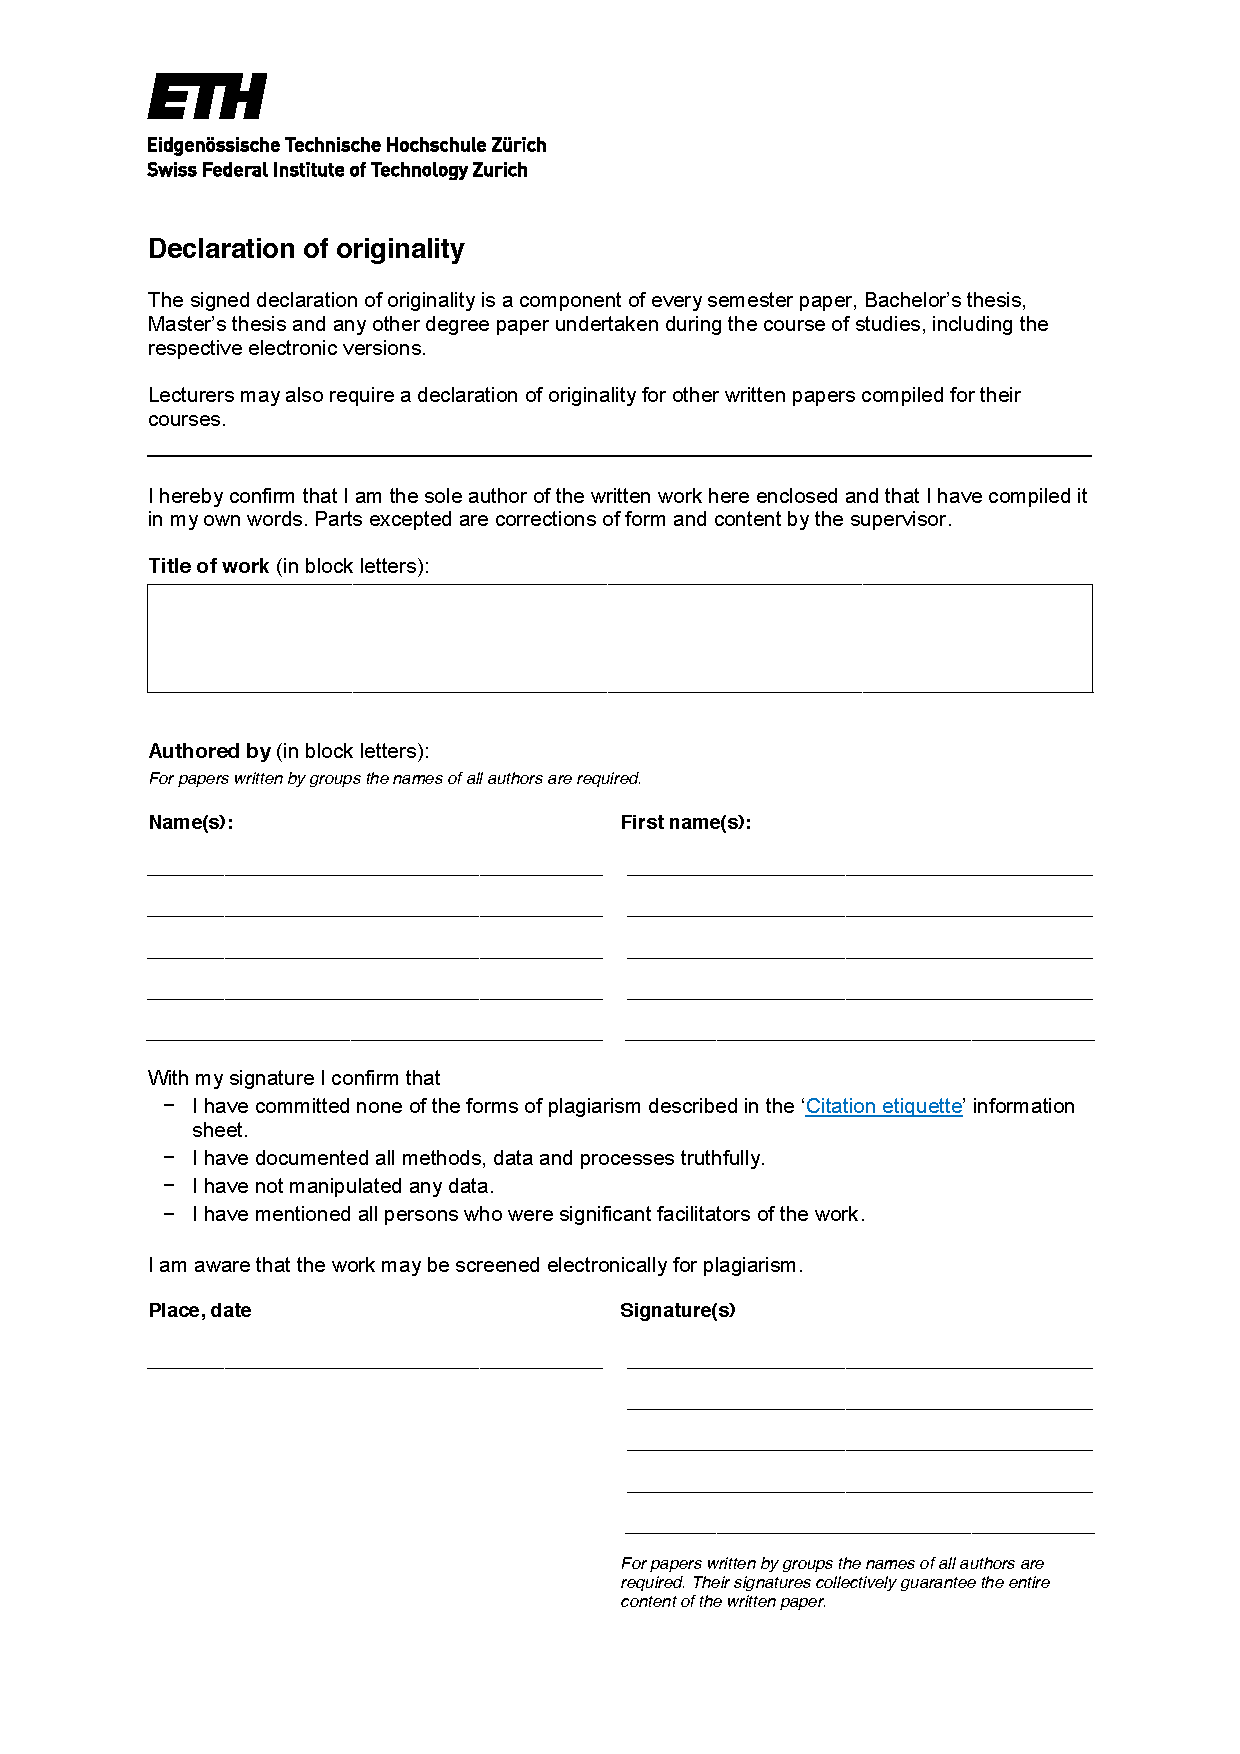
\includepdf[pages={-}]{declaration-originality.pdf}

\end{document}
